\begin{table*}[ht]
    \resizebox{\textwidth}{!}{
        \begin{tabular}{p{0.2\linewidth}|p{0.7\linewidth}}
        \toprule
           Product ID & Introduction \\
         \midrule
            B005NGQWL2 & Expand and accelerate your data transfer and charging. <br><br><b>The more the merrier.</b><br>With transfer rates of up to 5Gbps, set aside less time for syncing and more time for work. With 10 data terminals to choose from, forget about ever having to switch or unplug again.<br><br><b>Fast charging.</b><br>10th-port dual functionality enables fast charges of up to 1.5 amps with BC 1.2 charging-compliant devices, while simultaneously transferring data. Charge via a power adapter for higher 2 amp speeds with all USB-enabled devices when hub is disconnected from an active USB port, or your computer is off or in sleep mode. Dual functions, duly facilitated.<br><br><b>A mainstay for the future.</b><br>Featuring a high-grade chipset and a powerful 60W adapter, this hub ensures a stable power supply while you work. Get steady operation for years to come. Whether at home or in the office, add another can't-do-without fixture to your desk.<br><br><b>BC 1.2 Charging-Compliant Devices:</b><br>Apple: iPhone 5 / 5s, iPad Air, iPad mini / mini 2<br>Samsung: Galaxy S3 / S4, Galaxy Note 1 / 2, Galaxy Mega, Galaxy Mini, Exhilarate, Galaxy Tab 2 10.1<br>Google: Nexus 4 / 5 / 7 / 10<br>Sony: Xperia TX <br>Nokia: Lumia 920, Lumia 1020 <br><br><b>System Requirements</b><br>Windows (32/64 bit) 10 / 8.1 / 8 / 7 / Vista / XP, Mac OS X 10.6-10.9, Linux 2.6.14 or later.<br>Mac OS X Lion 10.7.4 users should upgrade to Mountain Lion 10.8.2 or later to avoid unstable connections.<br><br><b>Compatibility</b><br>2.4GHz wireless devices, MIDI devices and some USB 3.0 devices may not be supported. Try using the host port or a USB 2.0 connection.<br><br><b>Power Usage</b><br>For a stable connection, don't use this hub with high power-consumption devices, such as external hard drives. The hub will sync but not charge tablets and other devices which require a higher power input.

        \subfigure{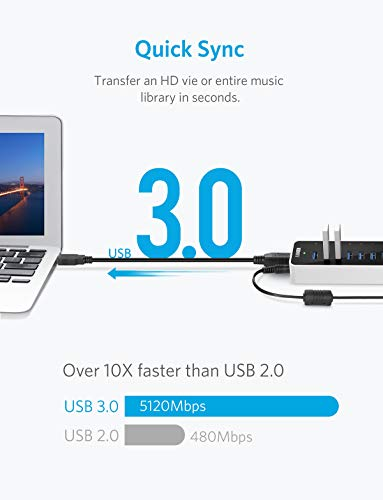
\includegraphics[height=\csfigheight]{Contents/img/case_study/product/pic_6_0.jpg}}
        \subfigure{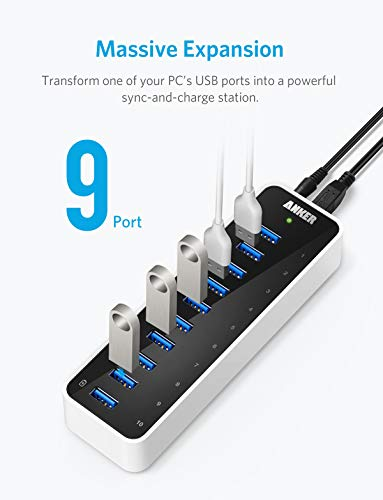
\includegraphics[height=\csfigheight]{Contents/img/case_study/product/pic_6_1.jpg}}
        \subfigure{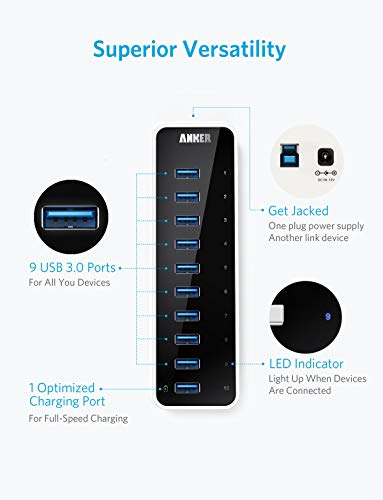
\includegraphics[height=\csfigheight]{Contents/img/case_study/product/pic_6_2.jpg}}
        \subfigure{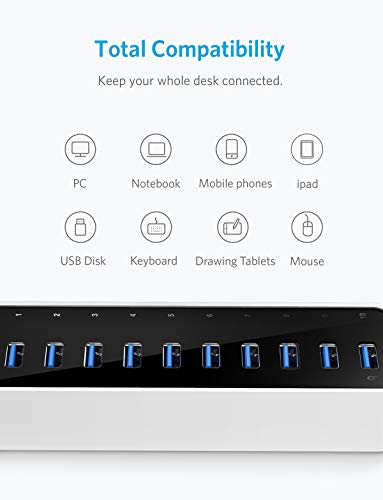
\includegraphics[height=\csfigheight]{Contents/img/case_study/product/pic_6_3.jpg}}
        \subfigure{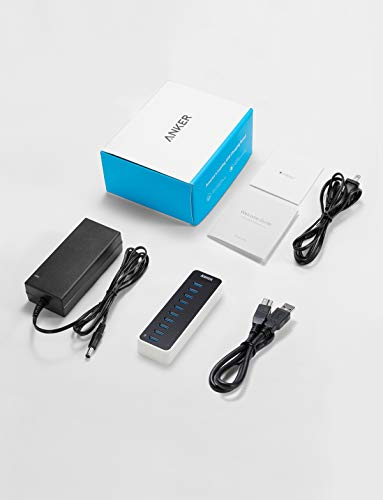
\includegraphics[height=\csfigheight]{Contents/img/case_study/product/pic_6_4.jpg}} 
        \subfigure{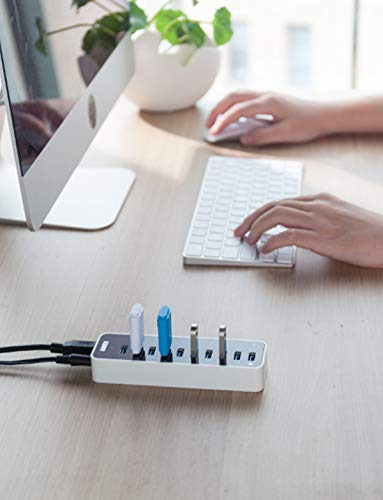
\includegraphics[height=\csfigheight]{Contents/img/case_study/product/pic_6_5.jpg}} 
        \\
        \bottomrule
        \end{tabular}
    }
    \caption{(Example 1 of 2) Product introduction of an example from Amazon Electronics dataset. Some special characters have been removed for better readability.}
    \label{tab:elec_product}
\end{table*}

\begin{table*}[ht!]
    \resizebox{\textwidth}{!}{
        \begin{tabular}{p{0.2\linewidth}|p{0.7\linewidth}|p{0.07\linewidth}|p{0.07\linewidth}|p{0.07\linewidth}}
        \toprule
        Review ID & Content & GT & GBDT & Ours \\
        \midrule
        B005NGQWL2-14 & 
        Pros:
        
        Has a nice look. Seems
        to work OK at full USB3 speeds. That's great since not all hubs do that.
        
        Cons: 

        Output is only 0.5A on the 10th data port as measured by an inline USB power meter while attempting to charge one of my Samsung tablets. I plugged that same tablet, cable and meter into a USB charger that DOES output the right current and the meter read 1.65A. 
        
        I am going to notify the seller about this and see what they have to say. Maybe I got one that has a problem? Who knows. 
        
        UPDATE: Received a replacement from the manufacturer. It has THE SAME PROBLEM: Port \#10 does NOT deliver 1.5A of charge current, even on the replacement they sent me. I even checked it against one of their other products, a 4 port charger which actually works correctly. See pictures. The first picture shows a USB power meter (``Eversame USB Digital Power Meter Tester Multimeter Current and Voltage Monitor") plugged into this hub into port \#10. It shows it charging my tablet at 0.42a. The second picture shows that same meter and same tablet plugged into the "Anker 36W 4-Port USB Wall Charger Travel Adapter with PowerIQ Technology" and charging at a normal 1.57a. Something is wrong here! I am contacting customer support line tomorrow to see what they want to do.
        
        \subfigure{
\includegraphics[height=\csfigheight]{Contents/img/case_study/review3/pic_2_0.jpg}}
        \subfigure{
\includegraphics[height=\csfigheight]{Contents/img/case_study/review3/pic_2_1.jpg}}
        & 3.00 & 0.86 & 0.89 \\
        \midrule
        B005NGQWL2-9 & I rarely write a negative review, in fact almost never. This AnkerDirect 10-Port USB Data hub lasted only about 2 months. Now none of the USB ports work.  For the first couple of weeks all the ports seemed fine. Then one by one they stopped working. Power gets to the unit and the USB ports on my MAC work fine. I've been waiting for a replacement from the company ever since April 20th 2017, after sending their support group my address as requested,  but it had not arrived.
        
        I wish to amend this review by saying that the Anker customer service folks were very helpful in rectifying this situation. After some checks on the original item at their direction, the Anker folks came to the conclusion that I had a defective product and quickly replaced it with a new model. I've had a couple of days to test it out and it appears to be working just fine. I have always felt that a product or service can go bad but it is the company's response to that problem, should it arise, that gains my respect and future business.

        \subfigure{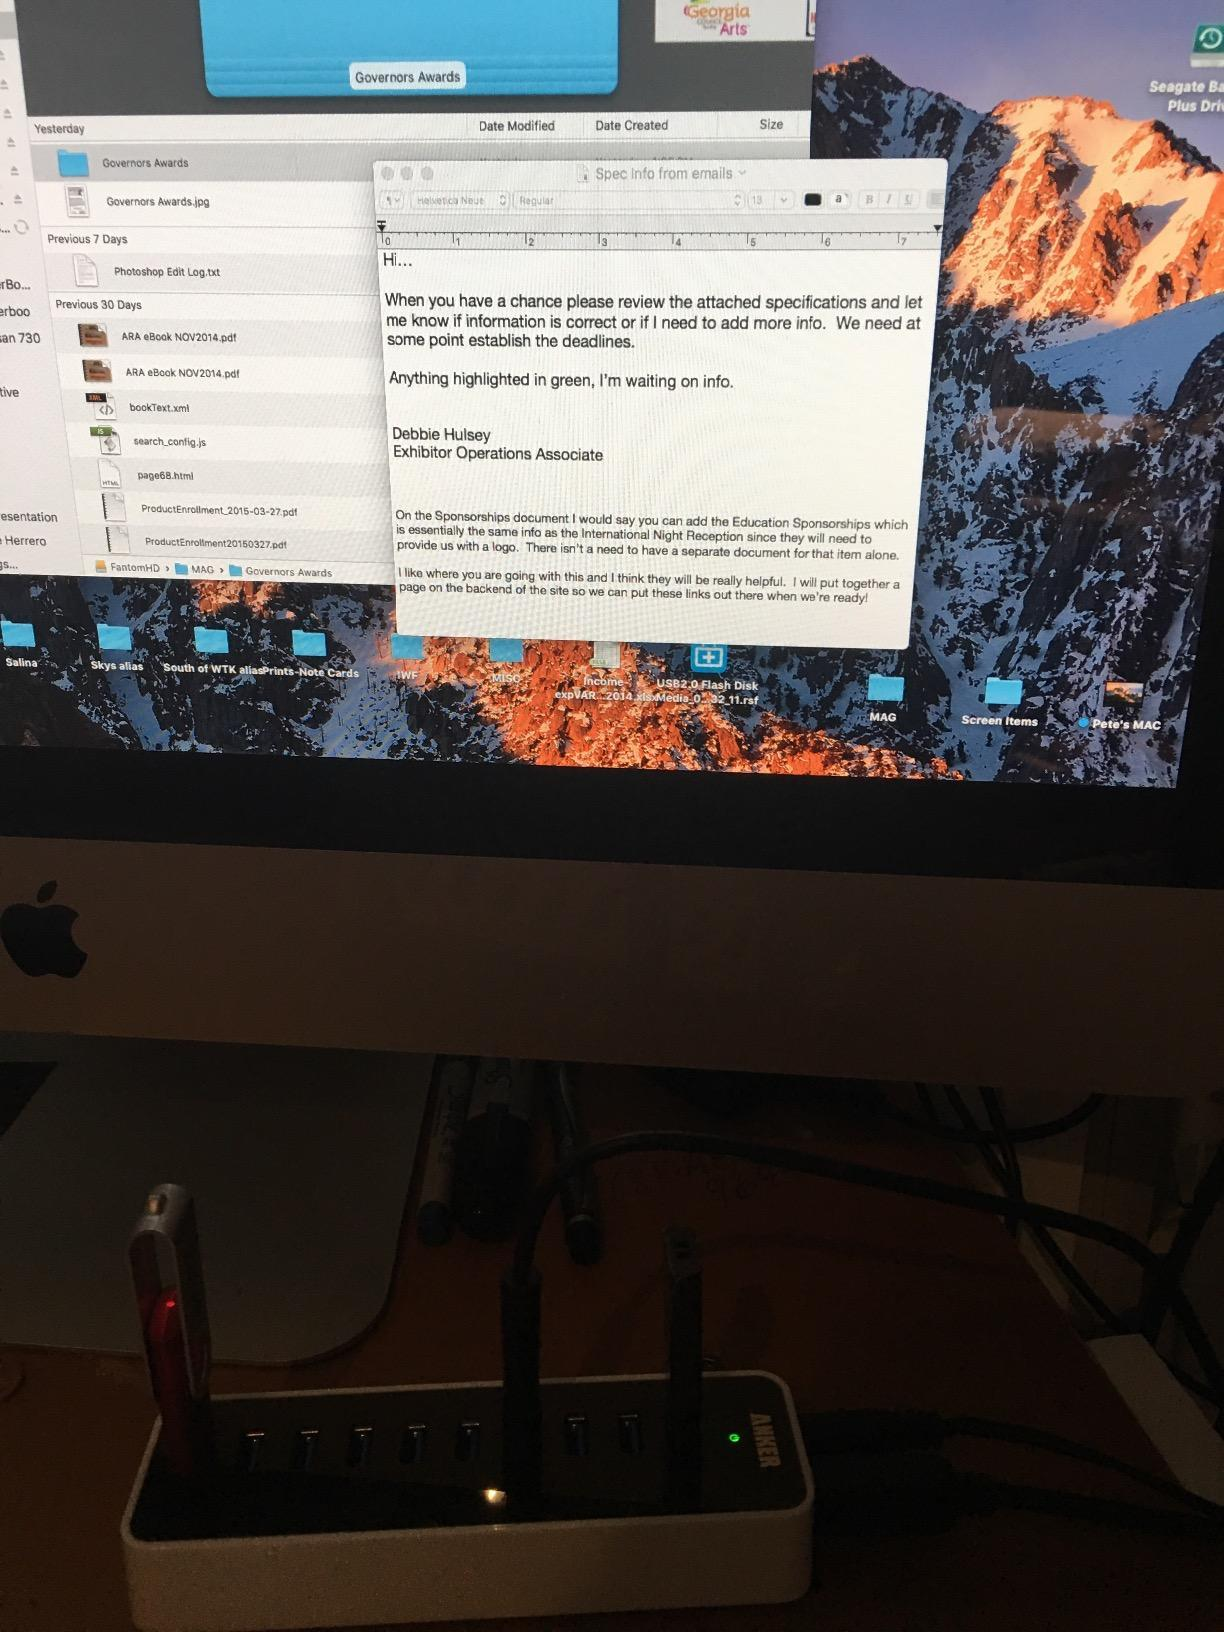
\includegraphics[height=\csfigheight]{Contents/img/case_study/review2/pic_1_0.jpg}}
        & 2.00 & 0.64 & 0.52 \\
        
        \midrule
        B005NGQWL2-65 & Works very great, powers all of my USB connections, I have a Asus Gaming Laptop which only has 4 USB ports and I needed to have a blue yeti mic, a Logitech Webcam c920,  razer keyboard chroma,  2tb hard drive,  and a Xbox one controller wireless adapter connected to it. 
        
        So far nothing has disconnected or malfunctioned. I would definitely recommend this to my friends and familiy. 
        
        \subfigure{
\includegraphics[height=\csfigheight]{Contents/img/case_study/review1/pic_2_0.jpg}}
        \subfigure{
\includegraphics[height=\csfigheight]{Contents/img/case_study/review1/pic_2_1.jpg}} & 1.00 & 0.75 & 0.31 \\
        \bottomrule
        \end{tabular}
    }
    \caption{(Example 1 of 2) Comparison between our model and GBDT on an example from Amazon electronics dataset. The ground truth (GT) scores are annotated ones, while the scores below GBDT and ours are normalized ones.}
    \label{tab:case_study1}
\end{table*}



\begin{table*}[ht!]
    \resizebox{\textwidth}{!}{
        \begin{tabular}{p{0.2\linewidth}|p{0.7\linewidth}}
        \toprule
           Product ID & Introduction \\
         \midrule
            B00H4O1L9Y & Cook food to perfection with the T-fal OptiGrill GC702D53 electric indoor grill. This indoor grill offers versatility and convenience for any grilled meals. Choose from six pre-set programs: Burger, Poultry, Sandwich, Sausage, Red Meat, and Fish. The grills precision grilling technology with sensors measures the thickness of food for auto cooking based on the program selected. When the flashing light turns solid purple, the grill has properly preheatedplace food on the grill, lower the lid, and it takes care of the rest. A cooking-level indicator light changes from yellow to orange to red signifying the cooking progress with audible beeps that alert when food gets to each stage: rare, medium, and well-done. Take food off the grill once its reached your preferred level of doneness. Along with the six pre-set programs, the electric grill provides two additional cooking options: Frozen mode for defrosting and fully cooking frozen food and Manual mode for cooking vegetables or personal recipes. (Note: when preheating for a pre-set program, keep the lid closed or the grill will automatically switch to Manual mode.) The OptiGrill features a powerful 1800-watt heating element, user-friendly controls ergonomically located on the handle, and die-cast aluminum plates with a nonstick coating for effortless food release. The slightly angled cooking plates allow fat to run away from food and into the drip tray for healthier results, and the drip tray and cooking plates are removable and dishwasher-safe for quick cleanup. Housed in brushed stainless steel, the OptiGrill electric indoor grill makes an attractive addition to any counter.  
    
            \subfigure{
\includegraphics[height=\csfigheight]{Contents/img/case_study2/product/pic_4_0.jpg}}
            \subfigure{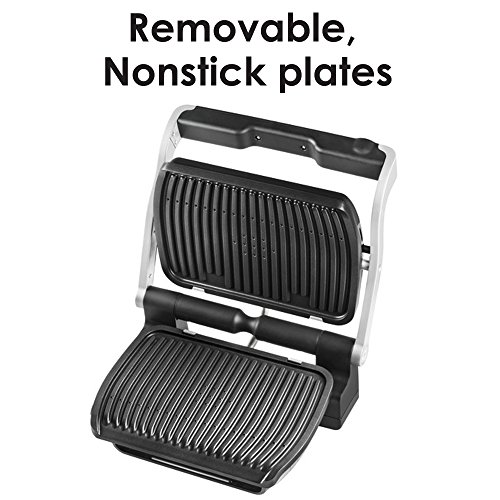
\includegraphics[height=\csfigheight]{Contents/img/case_study2/product/pic_4_1.jpg}}
            \subfigure{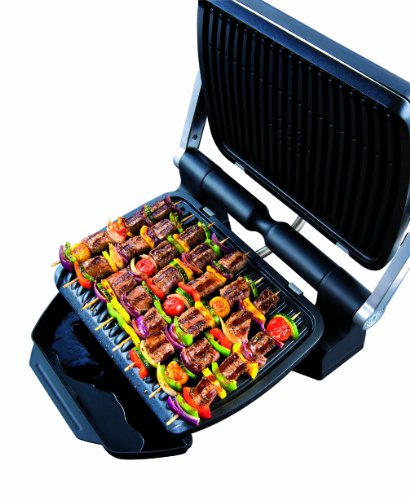
\includegraphics[height=\csfigheight]{Contents/img/case_study2/product/pic_4_2.jpg}}
            \subfigure{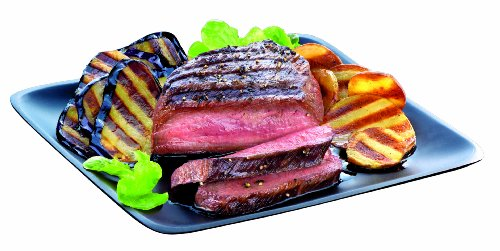
\includegraphics[height=\csfigheight]{Contents/img/case_study2/product/pic_4_3.jpg}} \\
        \bottomrule
        \end{tabular}
    }
    \caption{(Example 2 of 2) Product introduction of an example from Amazon Home dataset.}
    \label{tab:home_product}
\end{table*}

\begin{table*}[ht!]
    \resizebox{\textwidth}{!}{
        \begin{tabular}{p{0.2\linewidth}|p{0.7\linewidth}|p{0.07\linewidth}|p{0.07\linewidth}|p{0.07\linewidth}}
        \toprule
        Review ID & Content & GT & GBDT & Ours \\
        \midrule
        B00H4O1L9Y-111 & 
        I want to preface this by saying that I always prefer food grilled on our big outdoor propane grill.  It's just a superior method of cooking.  That being said, if you don't have an outdoor grill, or even if you do and are sometimes unable to cook with it due to lack of time, running out of propane, inclement weather, laziness...  then this is a FABULOUS option to still get the grilled food you loved SUPER FAST and SUPER EASY!!  We got 5 (yes FIVE) George Foreman grills for our wedding.  I re-gifted 4 of them and kept one and have used it off and on for a long time, but every time I have to clean it afterward I swear I'm never going to use it again because it's such a pain and it never quite gets clean, especially in the area where the hinges are.  That problem is no more....
        
        \subfigure{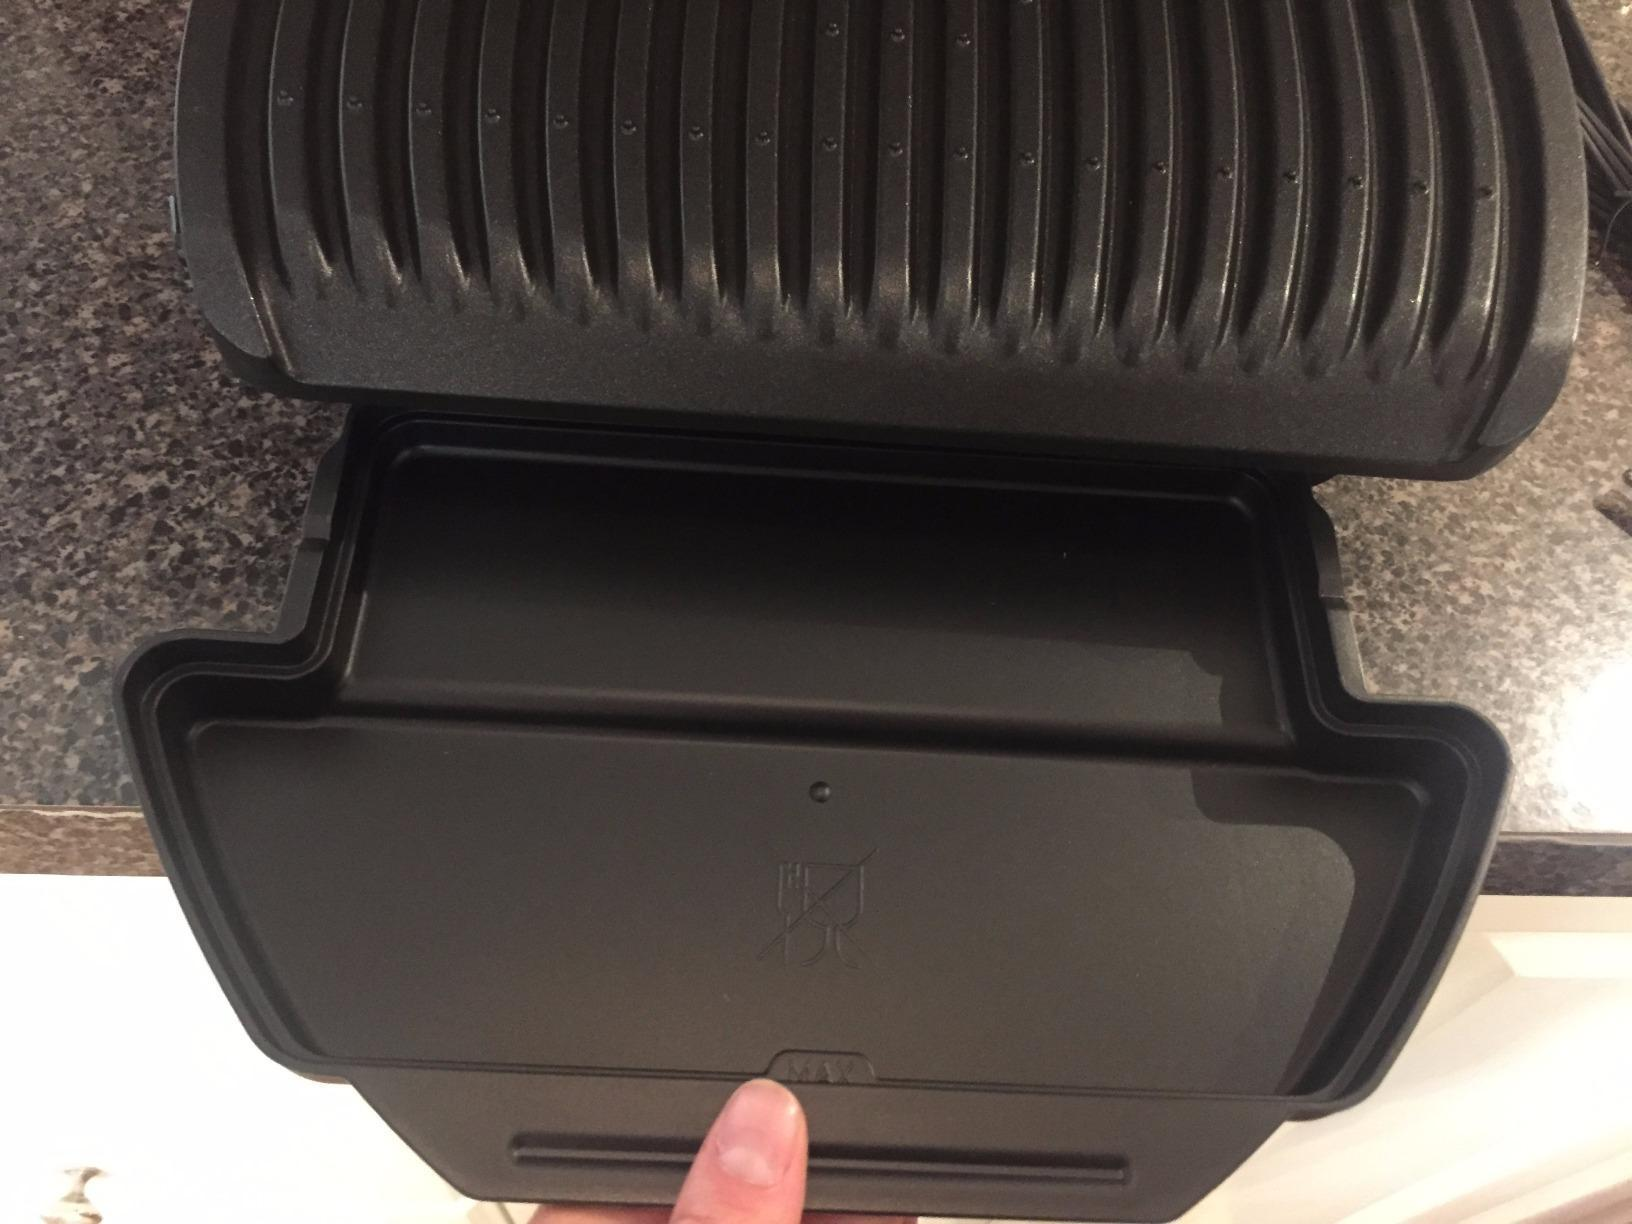
\includegraphics[height=\csfigheight]{Contents/img/case_study2/review4/pic_10_0.jpg}}
        \subfigure{
\includegraphics[height=\csfigheight]{Contents/img/case_study2/review4/pic_10_1.jpg}}
        \subfigure{
\includegraphics[height=\csfigheight]{Contents/img/case_study2/review4/pic_10_2.jpg}}
        \subfigure{
\includegraphics[height=\csfigheight]{Contents/img/case_study2/review4/pic_10_3.jpg}}
        \subfigure{
\includegraphics[height=\csfigheight]{Contents/img/case_study2/review4/pic_10_4.jpg}}
        \subfigure{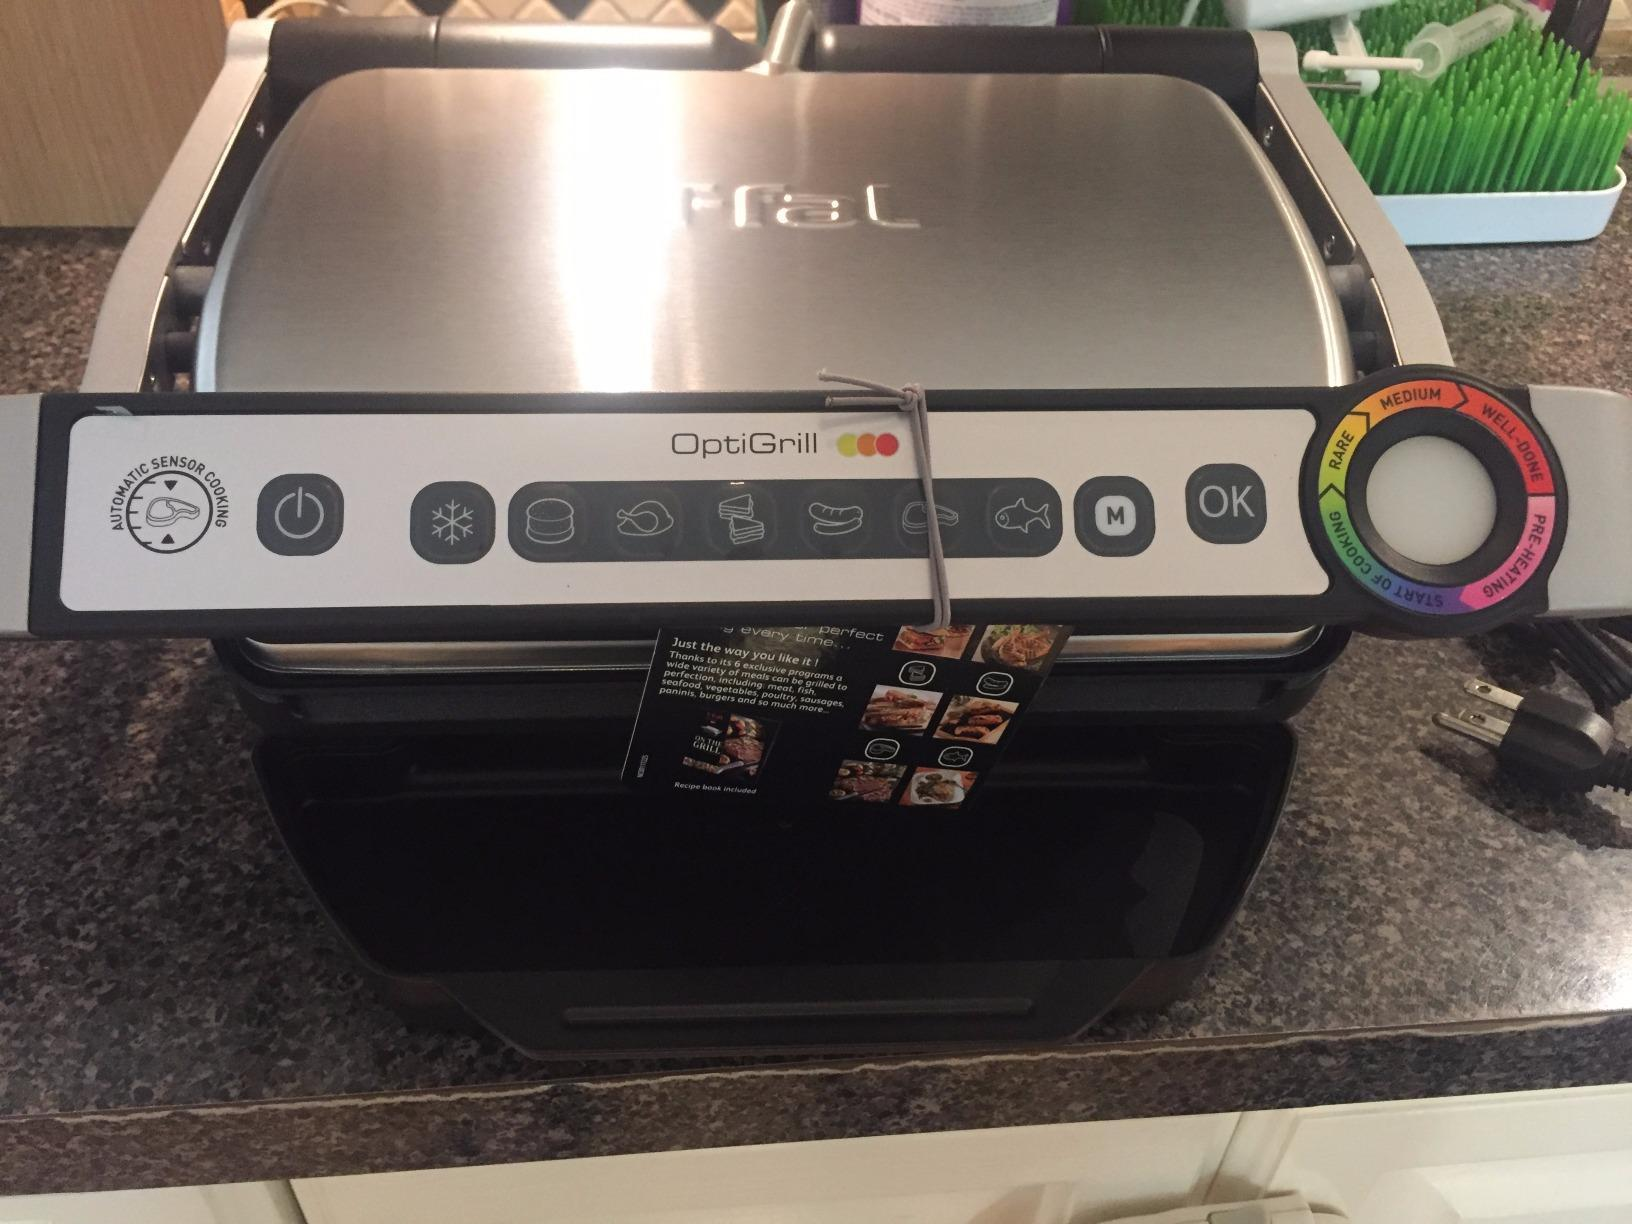
\includegraphics[height=\csfigheight]{Contents/img/case_study2/review4/pic_10_5.jpg}}
        \subfigure{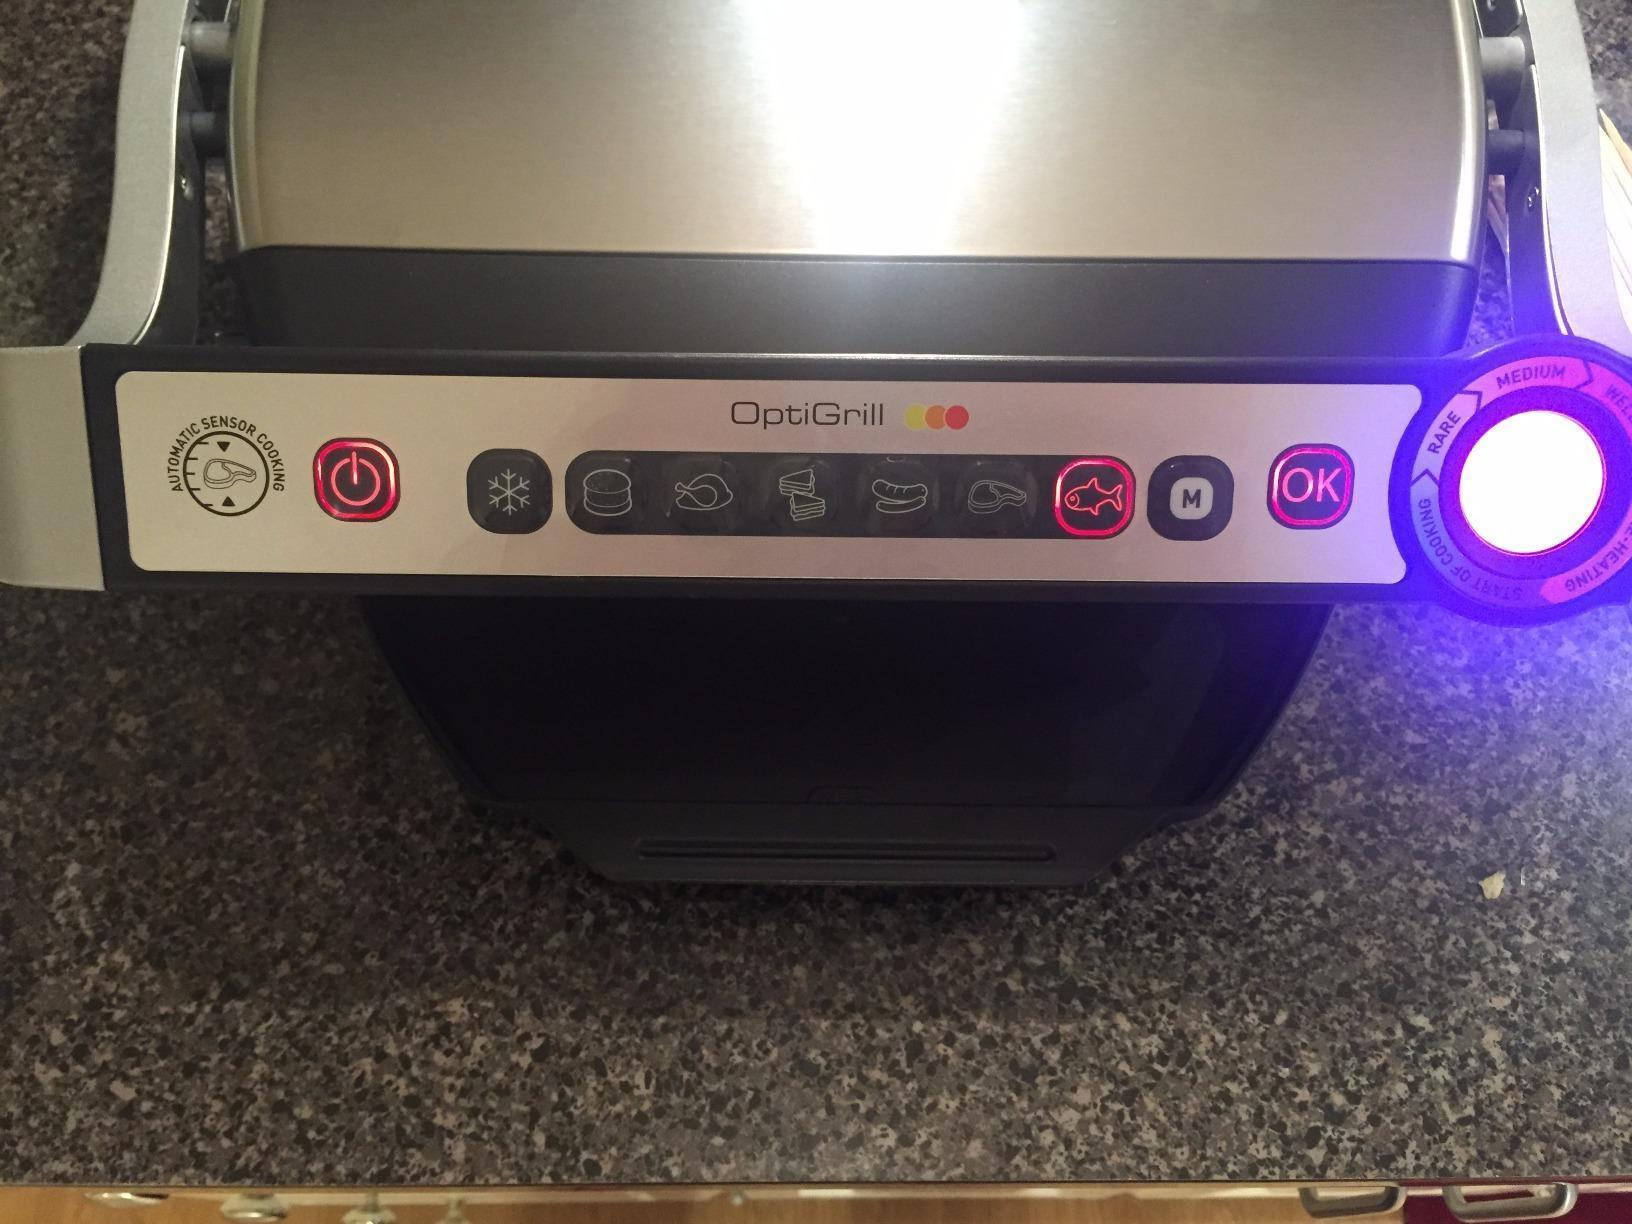
\includegraphics[height=\csfigheight]{Contents/img/case_study2/review4/pic_10_6.jpg}}
        & 4.00 & 0.58 & 0.71 \\
        \midrule
        B00H4O1L9Y-122   &
        My mom got this on her account. I thought she was crazy to spend so much on what looked like a glorified George Foreman grill but I was wrong, this thing is the bomb. Here is what I like about it;-Heats up super quick. I remember my old George Forman grill took a lot longer.-The presets for the type of food you are cooking must be working because nothing turns out overcooked.
        
        The nonstick removable plates. So far, I haven't had any food stick to the plates and I don't use spray or oil. Being able to take them off and wash them in the sink or dishwasher is by far the best part, I used to hate wasting a million paper towels and burning my hands on my old foreman grill and still didn't feel like it was clean. 
        
        Doesn't create a lot of smoke. When I used to use my old foreman grill I was always setting off the smoke alarm, this grill doesn't do that.
        
        \subfigure{
\includegraphics[height=\csfigheight]{Contents/img/case_study2/review3/pic_4_0.jpg}}
        \subfigure{
\includegraphics[height=\csfigheight]{Contents/img/case_study2/review3/pic_4_1.jpg}}
        \subfigure{
\includegraphics[height=\csfigheight]{Contents/img/case_study2/review3/pic_4_2.jpg}}
        \subfigure{
\includegraphics[height=\csfigheight]{Contents/img/case_study2/review3/pic_4_3.jpg}}
        & 3.00 & 0.65 & 0.62 \\
        
        \midrule
        B00H4O1L9Y-148 & I have used this grill 4 times now and everything I've cooked has turned out amazing! I am so impressed with this grill. It is real quick to preheat and has cooked everything perfectly so far from burgers to chicken sausages to kabobs. We haven't tried anything from the cookbook included but we definitely want to. One of the best things is that the plates are detachable and dishwasher safe! Super easy cleanup.
        
        \subfigure{
\includegraphics[height=\csfigheight]{Contents/img/case_study2/review2/pic_2_0.jpg}}
        \subfigure{
\includegraphics[height=\csfigheight]{Contents/img/case_study2/review2/pic_2_1.jpg}} & 2.00 & 0.49 & 0.42 \\
        \midrule
        B00H4O1L9Y-59 & One of the best tools for preparing clean food (if that's what you choose). Cooks in minutes and cleans just as fast. Gives that grill experience within a compact structure. Definitely saves time, I use this thing at least ounce a day, on prep days 3-5 times. If you want to loose wait; it starts in YOUR kitchen by preparing your meals. 
        
        \subfigure{
\includegraphics[height=\csfigheight]{Contents/img/case_study2/review1/pic_4_0.jpg}}
        \subfigure{
\includegraphics[height=\csfigheight]{Contents/img/case_study2/review1/pic_4_1.jpg}}
        \subfigure{
\includegraphics[height=\csfigheight]{Contents/img/case_study2/review1/pic_4_2.jpg}}
        \subfigure{
\includegraphics[height=\csfigheight]{Contents/img/case_study2/review1/pic_4_3.jpg}} & 1.00 & 0.35 & 0.27 \\
        \bottomrule
        \end{tabular}
    }
    \caption{(Example 2 of 2) Comparison between our model and GBDT on the example from Amazon Home dataset. The ground truth (GT) scores are annotated ones, while the scores below GBDT and ours are normalized ones.}
    \label{tab:case_study2}
\end{table*}